% -*- root: ../main.tex -*-
%!TEX root = ../main.tex
% this file is called up by main.tex
% content in this file will be fed into the main document
% vim:textwidth=80 fo=cqt

In this  section, the  quadratic approximation  of ionic  spatial concentration,
that underpins the electrolyte model  in many improved \gls{spm} formulations is
presented. An analysis of  the weakness of this model is  performed based on the
results  from applying  this model.  Mitigation of  this critical  drawback lead
to  this  author's  decoupled spatio-temporal  electrolyte  concentration  model
structure which is presented next in~\cref{sec:newelectrolytemodel}.

\begin{figure}[!htb]
    \captionsetup{singlelinecheck=off}
    \centering
    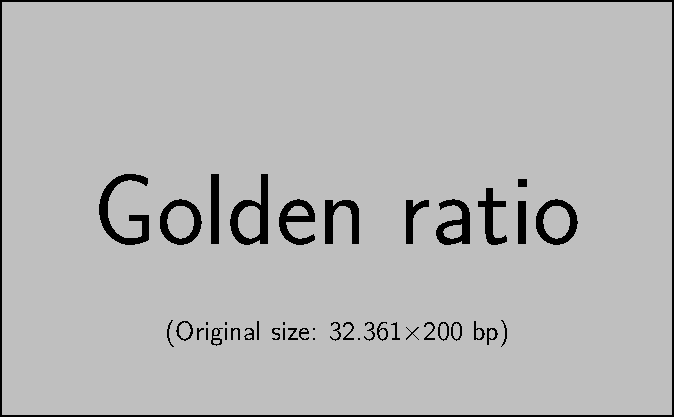
\includegraphics{placeholder_images/example-image-golden.pdf}
    \caption[Co-ordinate systems for quadratic approximation of
    electrolyte concentration]{Schematic diagram of the electrochemical sandwich
        consisting of
        \begin{enumerate*}[label=\itshape\alph*\upshape)]
            \item negative electrode,
            \item separator, and
            \item positive electrode
        \end{enumerate*} depicting the co-ordinate system used in deriving the
        quadratic approximation profile. The global spatial co-ordinate is $x
        \in \{0,l_\text{tot}\}$, where $l_\text{tot} = l_\text{neg} +
        l_\text{sep} + l_\text{pos}$. Local co-ordinate systems specific to each
        region are also defined. It should be noted that the positive
        electrode's local co-ordinate axis direction is reversed.}
    \label{fig:coordsquadapprox}
\end{figure}

The  schematic  in~\cref{fig:coordsquadapprox}  shows   the  definition  of  the
co-ordinate  systems  used  in  deriving the  polynomial  approximation  of  the
electrolyte concentration  profile. The globally defined  $x$ co-ordinate starts
at  the negative  current  collector  interface ($x=0$)  and  terminates at  the
positive  current  collector  interface  ($x =  l_\text{tot},\,  l_\text{tot}  =
l_\text{neg} +  l_\text{sep} +  l_\text{pos}$). Three local  co-ordinate systems
$z_\mu$  valid  only  within  their  respective regions  are  also  defined.  In
particular, it  must be  noted that  the direction  of the  local $z_\text{pos}$
co-ordinate axis is opposite to that of  the other two local co-ordinate axes as
well as the global co-ordinate axis. In subsequent usages, the suffix in $z_\mu$
is dropped and  the reader is advised  to infer the region of  validity from the
usage  context  which are  unambiguous  as  they  occur in  separate  equations.
Furthermore, the  notation of  the three regions  $\{\text{neg, sep,  pos}\}$ is
abbreviated  to $\{n,s,p\}$  respectively in  all mathematical  expressions. The
author  is convinced  that this  notation does  not detract  from following  the
derivations, but rather aids it by keeping the notations compact.

A  standard  quadratic expression  is  chosen  a  priori for  approximating  the
electrolyte concentration profile within each region.


% -*- root: ../main.tex -*-
%!TEX root = ../main.tex
% this file is called up by main.tex
% content in this file will be fed into the main document
% vim:nospell textwidth=180 foldlevelstart=3 foldlevel=3 conceallevel=0

\begin{table}[p]
    \centering
    \caption[Governing equations and boundary conditions of the \glsfmtshort{dfn} model]{Governing equations and boundary conditions of the \glsfmtlong{dfn} model}
    \label{tbl:dfneqns}
    \begingroup
    \makeatletter\def\f@size{9.8}\check@mathfonts
    \addtolength{\jot}{0.875em}
    \begin{tabular*}{\textwidth}{@{} l | l r l r @{}}
        \toprule
        \multicolumn{1}{c}{Region} & Governing equations & \multicolumn{2}{c}{Boundary conditions} & {} \\
        \midrule
    \multicolumn{1}{l |}{{\rotatebox[origin=c]{90}{\makecell{\footnotesize Separator\\ \scriptsize $\lambda \in \{\text{sep}\}$}}}} &
    % \multicolumn{3}{c}{\fbox{$ l_\text{neg} \coloneqq l_\text{n},\, l_\text{sep} \coloneqq l_\text{s},\, l_\text{pos} \coloneq l_\text{p}$}} &{} \\[0.5em]
    % {} &
    % $\begin{aligned}[t]
    %     \vphantom{\diffp{c_\text{e}}{x}{\mathrlap{x = l^{+}_\text{neg}}}} \varepsilon_\lambda \diffp{c_\text{e}}{t} &= \diffp{}{x}\left(D_\effmu \diffp{c_\text{e}}{x} \right) \\[-0.75em]
    % \end{aligned}$ &
    % $\begin{aligned}[t]
    % c_\text{e}\Bigr\rvert_{\mathrlap{x=l^{-}_\text{n}}}\hspace{5mm} &= c_\text{e}\Bigr\rvert_{\mathrlap{x=l^{+}_\text{n}}},\\[-0.75em]
    % c_\text{e}\Bigr\rvert_{\mathrlap{x=(l_{\text{n}} + l_\text{s})^{-}}}\hspace{5mm} &= c_\text{e}\Bigr\rvert_{\mathrlap{x=(l_{\text{n}} + l_\text{s})^{+}}},\\[1.25em]
    % \end{aligned}$ &
    % $\begin{aligned}[t]
    %     D_{\text{\tiny eff}_\text{n}}\!\! \! \!\, \diffp{c_\text{e}}{x}{\mathrlap{x = l^{-}_\text{n}}}\hspace{5mm} &=D_{\text{\tiny eff}_\text{s}}\!\!\!\!\,\diffp{c_\text{e}}{x}{\mathrlap{x = l^{+}_\text{n}}}\\[-0.75em]
    %     D_{\text{\tiny eff}_\text{s}}\!\! \! \!\, \diffp{c_\text{e}}{x}{\mathrlap{x=(l_{\text{n}} + l_\text{s})^{-}}}\hspace{5mm} &=D_{\text{\tiny eff}_\text{p}}\!\!\!\!\,\diffp{c_\text{e}}{x}{\mathrlap{x=(l_{\text{n}} + l_\text{s})^{+}}}\\[1.25em]
    % \end{aligned}$ &
    % $\begin{aligned}
    %     \refstepcounter{equation}(\theequation) \\[-0.75em]
    % \end{aligned}$
    % \\
    % {} &
    % $\begin{aligned}
    %     \frac{I}{A} &= \diffp{}{x}\left(\kappa_\effmu \diffp{\phi_\text{e}}{x}\right) + \diffp{}{x}\left(\kappa_\effmu \frac{2 R T(t)}{F} (t^0_{+}-1)\diffp{ \ln c_\text{e}}{x}\right) \\[-0.75em]
    % \end{aligned}$
    % & $\begin{aligned}[t]
    % \vphantom{\diffp{\phi_\text{e}}{x}{\mathrlap{x = l^{+}_\text{n}}}} \phi_\text{e}\Bigr\rvert_{\mathrlap{x=l^{-}_\text{n}}}\hspace{5mm} &= \phi_\text{e}\Bigr\rvert_{\mathrlap{x=l^{+}_\text{n}}},\\[-0.75em]
    % \phi_\text{e}\Bigr\rvert_{\mathrlap{x=(l_{\text{n}} + l_\text{s})^{-}}}\hspace{5mm} &= \phi_\text{e}\Bigr\rvert_{\mathrlap{x=(l_{\text{n}} + l_\text{s})^{-}}},\\
    % \end{aligned}$ &
    % $\begin{aligned}[t]
    %     \kappa_{\text{\tiny eff}_\text{n}}\!\! \! \!\, \diffp{c_\text{e}}{x}{\mathrlap{x = l^{-}_\text{n}}}\hspace{5mm} &=\kappa_{\text{\tiny eff}_\text{s}}\!\!\!\!\,\diffp{c_\text{e}}{x}{\mathrlap{x = l^{+}_\text{n}}}\\[-0.75em]
    %     \kappa_{\text{\tiny eff}_\text{s}}\!\! \! \!\, \diffp{c_\text{e}}{x}{\mathrlap{x=(l_{\text{n}} + l_\text{s})^{-}}}\hspace{5mm} &=\kappa_{\text{\tiny eff}_\text{p}}\!\!\!\!\,\diffp{c_\text{e}}{x}{\mathrlap{x=(l_{\text{n}} + l_\text{s})^{+}}}\\
    % \end{aligned}$ &
    % $\begin{aligned}
    %     \refstepcounter{equation}(\theequation) \\[-0.75em]
    % \end{aligned}$
    % \\
    \bottomrule
\end{tabular*}
\endgroup
\begin{minipage}{\textwidth}
    \bigskip
    \begin{flushleft}
        \raggedright
        \makeatletter\def\f@size{12}\check@mathfonts
        $ \text{\textbullet{} } c_\text{e}  \coloneqq c_\text{e}(x,t),\, \phi_\text{e} \coloneqq \phi_\text{e}(x,t) \quad \big\{\, x \in [0,l_\text{tot}],\, (x=0)\symbol{"2259} \text{\footnotesize neg/Cucc},\, (x=l_\text{tot})\symbol{"2259} \text{\footnotesize pos/Alcc}\, \big\}$
        \\[0.9em]
        {\raggedright \small \uline{\lambdainnegpos}}
        $\begin{alignedat}{2}
            & \text{\textbullet{} } c_\slambda & & \coloneqq c_\slambda(r,t),\, c_\slambdasurf \coloneqq c_\slambda(r=R_\plambda,t) \quad \big\{\, r \in [0,R_\plambda],\, (r=0)\symbol{"2259} \text{\footnotesize center},\, (r=R_\plambda)\symbol{"2259} \text{\footnotesize surface}\, \big\} \\[0.9em]
            % & \text{\textbullet{} } c_\slambdasurf & & \coloneqq c_\slambda(r=R_\plambda,t)\\
            & \text{\textbullet{} } \phi_\slambda & & \coloneqq \phi_\slambda(x_\lambda,t),\, j_\lambda \coloneqq j_\lambda(x_\lambda,t) \quad \big\{\, x_\lambda \subset x, \, x_\text{neg} \in [0,l_\text{pos}],\, x_\text{pos} \in [l_{\text{pos}+\text{neg}},l_\text{tot}]\, \big\} \\[0.9em]
            & \text{\textbullet{} } \eta_\lambda & & \coloneqq \eta_\lambda(x,t) = \phi_\slambda(x,t) - \phi_\text{e}(x,t) - \mathcal{U}_\lambda(c_\slambdasurf) \\
            & \text{\textbullet{} } \sigma_\efflambda & & = \sigma_\lambda \varepsilon_\slambda,\, D_\sefflambda = D_\slambda e^{\frac{-E_{\text{a},D_\slambda}}{R}\left(\frac{1}{T(t)} - \frac{1}{T_\text{sink}}\right)},\, k_\refflambda = k_\lambdar e^{\frac{-E_{\text{a},k_\lambdar}}{R}\left(\frac{1}{T(t)} - \frac{1}{T_\text{sink}}\right)} \\[0.9em]
        \end{alignedat}$
        {\raggedright \small \uline{\muinnegseppos}}\\[0.5ex]
        $\begin{alignedat}{2}
            & \text{\textbullet{} } D_\effmu & & = D \varepsilon_\lambda^{\text{brugg}_\lambda} \\
            & \text{\textbullet{} } D & & \coloneqq D(\scriptstyle{c_\text{e},T}\,\textstyle) = 10^{-4} \times 10^{-4.43 - \frac{54}{T(t) - 229 - 5\times10^{-3} c_\text{e}(x,t)} - 0.22\times10^{-3} c_\text{e}(x,t)} \\
        \end{alignedat}$
        \\
        \makeatletter\def\f@size{14}\check@mathfonts
        $\begin{alignedat}{2}
            & \text{\textbullet{} } \kappa_\effmu & & = \kappa \varepsilon_\lambda^{\text{brugg}_\lambda} \\
            & \text{\textbullet{} } \kappa & & \coloneqq \kappa\scriptstyle{(c_\text{e},T)}\; = \; \parbox[t]{11.60cm}{$\scriptstyle 10^{-4} \times c_\text{e}(x,t)\Big(-10.5 + 0.668\times10^{-3} c_\text{e}(x,t) + 0.494\times10^{-6} c_\text{e}^2(x,t) + \big(0.074 - 1.78\times10^{-5}c_\text{e}(x,t)$ \\ \hspace*{\fill} $\scriptstyle - 8.86\times10^{-10}c_\text{e}^2(x,t)\big)T(t) + \big(-6.96\times10^{-5} + 2.8\times10^{-8} c_\text{e}(x,t)\big)T^2(t)\Big)^2$}\\
        \end{alignedat}$
    \end{flushleft}
\end{minipage}
\end{table}


